

\tikzset{every picture/.style={line width=0.75pt}} %set default line width to 0.75pt        

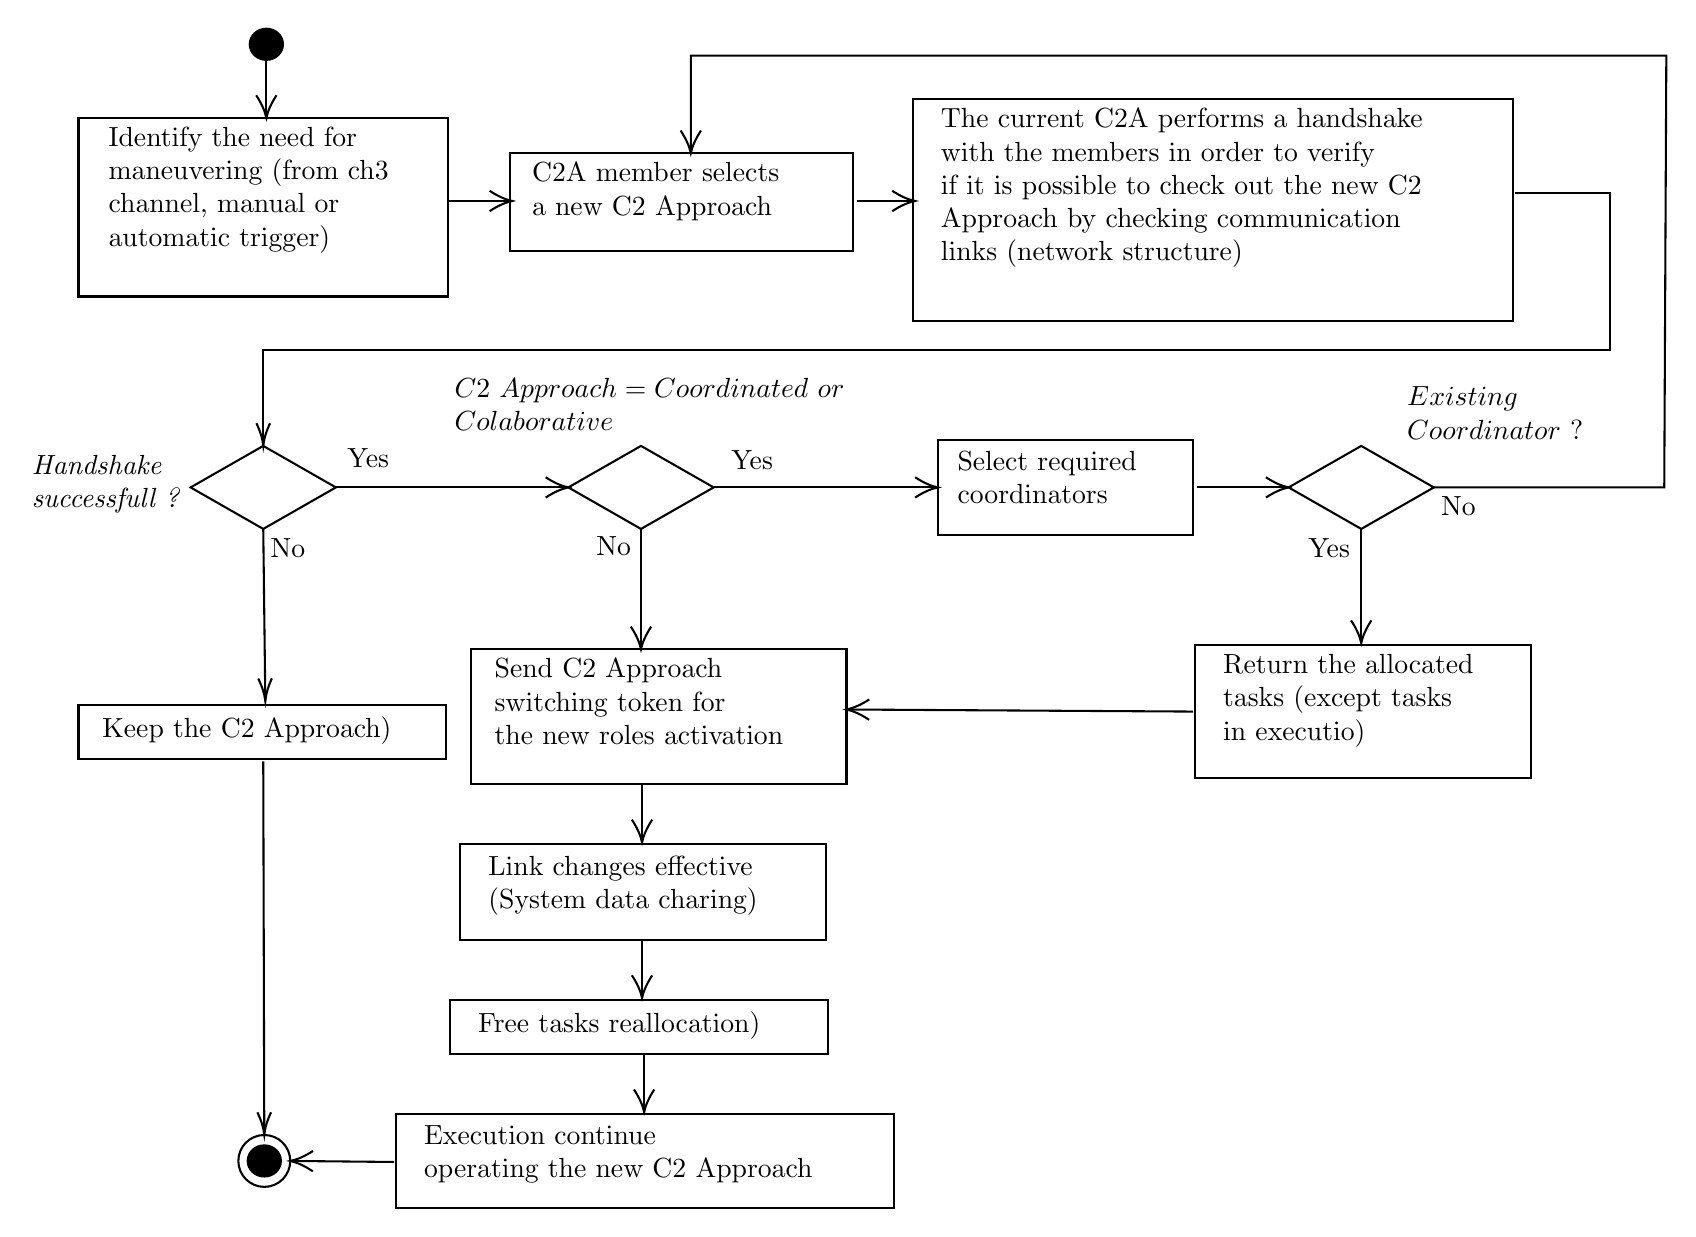
\begin{tikzpicture}[x=0.75pt,y=0.75pt,yscale=-1,xscale=1]
%uncomment if require: \path (0,587); %set diagram left start at 0, and has height of 587

%Flowchart: Connector [id:dp30004727364023565] 
\draw  [fill={rgb, 255:red, 0; green, 0; blue, 0 }  ,fill opacity=1 ] (107.5,15.5) .. controls (107.5,11.36) and (111.08,8) .. (115.5,8) .. controls (119.92,8) and (123.5,11.36) .. (123.5,15.5) .. controls (123.5,19.64) and (119.92,23) .. (115.5,23) .. controls (111.08,23) and (107.5,19.64) .. (107.5,15.5) -- cycle ;
%Flowchart: Process [id:dp49355233268787946] 
\draw   (25,51) -- (203,51) -- (203,137) -- (25,137) -- cycle ;
%Flowchart: Process [id:dp5792314547374635] 
\draw   (233,68) -- (398,68) -- (398,115) -- (233,115) -- cycle ;
%Flowchart: Decision [id:dp6129764683030855] 
\draw   (296,209) -- (331,229) -- (296,249) -- (261,229) -- cycle ;
%Flowchart: Process [id:dp06845031700936466] 
\draw   (439,206) -- (562,206) -- (562,252) -- (439,252) -- cycle ;
%Flowchart: Decision [id:dp49593776360146347] 
\draw   (643,209) -- (678,229) -- (643,249) -- (608,229) -- cycle ;
%Flowchart: Process [id:dp6261439474780552] 
\draw   (214,307) -- (395,307) -- (395,372) -- (214,372) -- cycle ;
%Flowchart: Process [id:dp5086061580242806] 
\draw   (209,401) -- (385,401) -- (385,447) -- (209,447) -- cycle ;
%Flowchart: Process [id:dp8537911496336553] 
\draw   (204,476) -- (386,476) -- (386,502) -- (204,502) -- cycle ;
%Flowchart: Process [id:dp6544494461524978] 
\draw   (178,531) -- (418,531) -- (418,576) -- (178,576) -- cycle ;
%Flowchart: Connector [id:dp871332920123143] 
\draw  [fill={rgb, 255:red, 0; green, 0; blue, 0 }  ,fill opacity=1 ] (106.5,553.5) .. controls (106.5,549.36) and (110.08,546) .. (114.5,546) .. controls (118.92,546) and (122.5,549.36) .. (122.5,553.5) .. controls (122.5,557.64) and (118.92,561) .. (114.5,561) .. controls (110.08,561) and (106.5,557.64) .. (106.5,553.5) -- cycle ;
%Shape: Circle [id:dp2271913054537874] 
\draw   (102,553.5) .. controls (102,546.6) and (107.6,541) .. (114.5,541) .. controls (121.4,541) and (127,546.6) .. (127,553.5) .. controls (127,560.4) and (121.4,566) .. (114.5,566) .. controls (107.6,566) and (102,560.4) .. (102,553.5) -- cycle ;

%Straight Lines [id:da5553992976930034] 
\draw    (115.5,23) -- (115.5,49) ;
\draw [shift={(115.5,51)}, rotate = 270] [color={rgb, 255:red, 0; green, 0; blue, 0 }  ][line width=0.75]    (10.93,-4.9) .. controls (6.95,-2.3) and (3.31,-0.67) .. (0,0) .. controls (3.31,0.67) and (6.95,2.3) .. (10.93,4.9)   ;
%Straight Lines [id:da5603484879152818] 
\draw    (203,91) -- (232,91) ;
\draw [shift={(234,91)}, rotate = 180] [color={rgb, 255:red, 0; green, 0; blue, 0 }  ][line width=0.75]    (10.93,-4.9) .. controls (6.95,-2.3) and (3.31,-0.67) .. (0,0) .. controls (3.31,0.67) and (6.95,2.3) .. (10.93,4.9)   ;
%Straight Lines [id:da6509051861301578] 
\draw    (400,91) -- (426,91) ;
\draw [shift={(428,91)}, rotate = 180] [color={rgb, 255:red, 0; green, 0; blue, 0 }  ][line width=0.75]    (10.93,-4.9) .. controls (6.95,-2.3) and (3.31,-0.67) .. (0,0) .. controls (3.31,0.67) and (6.95,2.3) .. (10.93,4.9)   ;
%Straight Lines [id:da8066330051931784] 
\draw    (149,229) -- (259,229) ;
\draw [shift={(261,229)}, rotate = 180] [color={rgb, 255:red, 0; green, 0; blue, 0 }  ][line width=0.75]    (10.93,-4.9) .. controls (6.95,-2.3) and (3.31,-0.67) .. (0,0) .. controls (3.31,0.67) and (6.95,2.3) .. (10.93,4.9)   ;
%Straight Lines [id:da8032694301364721] 
\draw    (564,229) -- (606,229) ;
\draw [shift={(608,229)}, rotate = 180] [color={rgb, 255:red, 0; green, 0; blue, 0 }  ][line width=0.75]    (10.93,-4.9) .. controls (6.95,-2.3) and (3.31,-0.67) .. (0,0) .. controls (3.31,0.67) and (6.95,2.3) .. (10.93,4.9)   ;
%Straight Lines [id:da27464611431635977] 
\draw    (331,229) -- (437,229) ;
\draw [shift={(439,229)}, rotate = 180] [color={rgb, 255:red, 0; green, 0; blue, 0 }  ][line width=0.75]    (10.93,-4.9) .. controls (6.95,-2.3) and (3.31,-0.67) .. (0,0) .. controls (3.31,0.67) and (6.95,2.3) .. (10.93,4.9)   ;
%Straight Lines [id:da2782211155026265] 
\draw    (296.5,372) -- (296.5,398) ;
\draw [shift={(296.5,400)}, rotate = 270] [color={rgb, 255:red, 0; green, 0; blue, 0 }  ][line width=0.75]    (10.93,-4.9) .. controls (6.95,-2.3) and (3.31,-0.67) .. (0,0) .. controls (3.31,0.67) and (6.95,2.3) .. (10.93,4.9)   ;
%Straight Lines [id:da2251054003440185] 
\draw    (296.5,447) -- (296.5,473) ;
\draw [shift={(296.5,475)}, rotate = 270] [color={rgb, 255:red, 0; green, 0; blue, 0 }  ][line width=0.75]    (10.93,-4.9) .. controls (6.95,-2.3) and (3.31,-0.67) .. (0,0) .. controls (3.31,0.67) and (6.95,2.3) .. (10.93,4.9)   ;
%Straight Lines [id:da630379124340155] 
\draw    (297.5,502) -- (297.5,528) ;
\draw [shift={(297.5,530)}, rotate = 270] [color={rgb, 255:red, 0; green, 0; blue, 0 }  ][line width=0.75]    (10.93,-4.9) .. controls (6.95,-2.3) and (3.31,-0.67) .. (0,0) .. controls (3.31,0.67) and (6.95,2.3) .. (10.93,4.9)   ;
%Straight Lines [id:da9050309983342688] 
\draw    (177,554) -- (129,553.52) ;
\draw [shift={(127,553.5)}, rotate = 360.57] [color={rgb, 255:red, 0; green, 0; blue, 0 }  ][line width=0.75]    (10.93,-4.9) .. controls (6.95,-2.3) and (3.31,-0.67) .. (0,0) .. controls (3.31,0.67) and (6.95,2.3) .. (10.93,4.9)   ;
%Straight Lines [id:da21363668845567407] 
\draw    (562,337) -- (397,336.01) ;
\draw [shift={(395,336)}, rotate = 360.34000000000003] [color={rgb, 255:red, 0; green, 0; blue, 0 }  ][line width=0.75]    (10.93,-4.9) .. controls (6.95,-2.3) and (3.31,-0.67) .. (0,0) .. controls (3.31,0.67) and (6.95,2.3) .. (10.93,4.9)   ;
%Straight Lines [id:da3585668105072546] 
\draw    (643,249) -- (643,302) ;
\draw [shift={(643,304)}, rotate = 270] [color={rgb, 255:red, 0; green, 0; blue, 0 }  ][line width=0.75]    (10.93,-4.9) .. controls (6.95,-2.3) and (3.31,-0.67) .. (0,0) .. controls (3.31,0.67) and (6.95,2.3) .. (10.93,4.9)   ;
%Straight Lines [id:da9657566875951242] 
\draw    (296,249) -- (296,305) ;
\draw [shift={(296,307)}, rotate = 270] [color={rgb, 255:red, 0; green, 0; blue, 0 }  ][line width=0.75]    (10.93,-4.9) .. controls (6.95,-2.3) and (3.31,-0.67) .. (0,0) .. controls (3.31,0.67) and (6.95,2.3) .. (10.93,4.9)   ;
%Straight Lines [id:da8958852215420727] 
\draw    (114,249) -- (114.98,330) ;
\draw [shift={(115,332)}, rotate = 269.31] [color={rgb, 255:red, 0; green, 0; blue, 0 }  ][line width=0.75]    (10.93,-3.29) .. controls (6.95,-1.4) and (3.31,-0.3) .. (0,0) .. controls (3.31,0.3) and (6.95,1.4) .. (10.93,3.29)   ;
%Straight Lines [id:da4274455247533797] 
\draw    (114,361) -- (114.49,539) ;
\draw [shift={(114.5,541)}, rotate = 269.84000000000003] [color={rgb, 255:red, 0; green, 0; blue, 0 }  ][line width=0.75]    (10.93,-3.29) .. controls (6.95,-1.4) and (3.31,-0.3) .. (0,0) .. controls (3.31,0.3) and (6.95,1.4) .. (10.93,3.29)   ;
%Shape: Rectangle [id:dp719664176394256] 
\draw   (427,42) -- (716,42) -- (716,149) -- (427,149) -- cycle ;
%Flowchart: Decision [id:dp9069295799748449] 
\draw   (114,209) -- (149,229) -- (114,249) -- (79,229) -- cycle ;
%Straight Lines [id:da5931871136517136] 
\draw    (717,87) -- (763,87) -- (763,163) -- (114,163) -- (114,207) ;
\draw [shift={(114,209)}, rotate = 270] [color={rgb, 255:red, 0; green, 0; blue, 0 }  ][line width=0.75]    (10.93,-3.29) .. controls (6.95,-1.4) and (3.31,-0.3) .. (0,0) .. controls (3.31,0.3) and (6.95,1.4) .. (10.93,3.29)   ;
%Flowchart: Process [id:dp8465302396716761] 
\draw   (563,305) -- (725,305) -- (725,369) -- (563,369) -- cycle ;
%Straight Lines [id:da6376219841774388] 
\draw    (678,229) -- (789,229) -- (790,21) -- (320,21) -- (320,66) ;
\draw [shift={(320,68)}, rotate = 270] [color={rgb, 255:red, 0; green, 0; blue, 0 }  ][line width=0.75]    (10.93,-4.9) .. controls (6.95,-2.3) and (3.31,-0.67) .. (0,0) .. controls (3.31,0.67) and (6.95,2.3) .. (10.93,4.9)   ;
%Flowchart: Process [id:dp8368851607381006] 
\draw   (25,334) -- (202,334) -- (202,360) -- (25,360) -- cycle ;

% Text Node
\draw (198,173) node [anchor=north west][inner sep=0.75pt]    {$ \begin{array}{l}
C2\ Approach=Coordinated\ or\ \\
Colaborative
\end{array}$};
% Text Node
\draw (657,177) node [anchor=north west][inner sep=0.75pt]    {$ \begin{array}{l}
Existing\\
Coordinator\ ?
\end{array}$};
% Text Node
\draw (190,535) node [anchor=north west][inner sep=0.75pt]   [align=left] {Execution continue \\operating the new C2 Approach};
% Text Node
\draw (338,210) node [anchor=north west][inner sep=0.75pt]   [align=left] {Yes};
% Text Node
\draw (273,251) node [anchor=north west][inner sep=0.75pt]   [align=left] {No};
% Text Node
\draw (616,252) node [anchor=north west][inner sep=0.75pt]   [align=left] {Yes};
% Text Node
\draw (1,212) node [anchor=north west][inner sep=0.75pt]   [align=left] {\textit{Handshake}\\\textit{successfull ?}};
% Text Node
\draw (38,54) node [anchor=north west][inner sep=0.75pt]   [align=left] {Identify the need for \\maneuvering (from ch3\\channel, manual or \\automatic trigger)};
% Text Node
\draw (242,71) node [anchor=north west][inner sep=0.75pt]   [align=left] {C2A member selects \\a new C2 Approach};
% Text Node
\draw (439,45) node [anchor=north west][inner sep=0.75pt]   [align=left] {The current C2A performs a handshake\\with the members in order to verify\\if it is possible to check out the new C2 \\Approach by checking communication\\links (network structure)};
% Text Node
\draw (116,252) node [anchor=north west][inner sep=0.75pt]   [align=left] {No};
% Text Node
\draw (153,209) node [anchor=north west][inner sep=0.75pt]   [align=left] {Yes};
% Text Node
\draw (447,210) node [anchor=north west][inner sep=0.75pt]   [align=left] {Select required \\coordinators};
% Text Node
\draw (575,308) node [anchor=north west][inner sep=0.75pt]   [align=left] {Return the allocated\\tasks (except tasks\\in executio) };
% Text Node
\draw (224,310) node [anchor=north west][inner sep=0.75pt]   [align=left] {Send C2 Approach \\switching token for \\the new roles activation};
% Text Node
\draw (680,232) node [anchor=north west][inner sep=0.75pt]   [align=left] {No};
% Text Node
\draw (221,405) node [anchor=north west][inner sep=0.75pt]   [align=left] {Link changes effective\\(System data charing)};
% Text Node
\draw (216,480) node [anchor=north west][inner sep=0.75pt]   [align=left] {Free tasks reallocation)};
% Text Node
\draw (35,338) node [anchor=north west][inner sep=0.75pt]   [align=left] {Keep the C2 Approach)};


\end{tikzpicture}